%-------------------------------------------------------------------
%2013-04-23  toph  FOR NOW COMMENTED OUT ADDITIONAL SLIDES SECTIONS

% \section{Additional Slides}

% \subsection{AID Stability Analysis}

% \begin{frame}[t]{Rigid Body Model}
%   \begin{align} 
%     \uncover<1>{\dot{R}(t)}&\uncover<1>{=R(t)\mathcal{J}(\omega(t))}
%     \nonumber \\
%     I\dot{\omega}(t)&=\mathcal{J}(I\omega(t))\omega(t)
%     \uncover<1>{+\left(\sum_{i=1}^3 |\omega_i|C_i
%     \right)\omega(t)+\mathcal{J}(b)R(t)^T e_3}+u(t)
%     \nonumber 
%  \end{align}

%  \begin{itemize}
%    \item<2-> Standard Second Order Rotating Rigid Body System 
%    \item<3-> Typically used to model satellites
%    \item<4-> We first developed an Adaptive Identifier for this system first
%  \end{itemize}

% \end{frame}


% \begin{frame}{Rigid Body Adaptive Identification}

%   \begin{columns}
%     \column{.32\textwidth}

%     Error Coordinates:
%     \begin{align}
%       \Delta\omega(t)&=\hat{\omega}(t)-\omega(t)  \nonumber \\
%       \Delta I(t)&=\hat{I}(t) - I                 \nonumber
%     \end{align}
    
%     System:
%     \begin{equation*}
%       \dot{\omega} =I^{-1}\left(\mathcal{J}(I\omega)\omega+u\right) 
%     \end{equation*}
    
%     Adaptive Identifier:
%     \begin{align}
%       \dot{\hat{\omega}}=&\hat{I}^{-1}\left(
%         \mathcal{J}(\hat{I}\omega)\omega
%         + u\right) - a \Delta \omega    \nonumber \\
%       \dot{\hat{I}}=&-\frac{1}{2}\left(\psi_1 \omega^T +\omega
%         \psi_1^T\right)
%       \nonumber \\
%       &+\frac{1}{2}\left(\Delta\omega \psi_2^T+\psi_2
%         \Delta\omega^T\right)\only<5>{.}  \nonumber
%     \end{align}
    
%     \pause
    
%     \column{.68\textwidth}
%     \temporal<3>
%     {with the following constraints:
%       \begin{itemize}
%       \item $u(t)$ and $\omega(t)$ bounded by assumption
%       \item $a\in\mathbb{R}_+$
%       \item $\psi_1=\mathcal{J}(\omega)\Delta \omega$
%       \item
%         $\psi_2=\hat{I}^{-1}\left(\mathcal{J}\left(\hat{I}\omega\right)
%           \omega +u\right)$
%       \item $\hat{I}(t_0)$ is SPD
%       \item $\hat{\omega}(t_0)=\omega(t_0)$
%       \item $\exists \epsilon \in \mathbb{R}_+$ such that $\|\Delta
%         I(t_0)\|_F+\epsilon \leq \lambda_3$
%       \end{itemize}
      
%     }{ 
      
%       %\color{green}{Lyapunov Stability Proof Outline}
%       %Lyapunov Stability Proof Outline
%       Error Dynamics:
%       \begin{align}
%         \dot{\Delta I}&=-\frac{1}{2}\left(\psi_1 \omega^T +\omega
%           \psi_1^T -\Delta\omega \psi_2^T-\psi_2 \Delta\omega^T\right)
%         \nonumber \\
%         \dot{\Delta \omega}&=-I^{-1}\left(a I
%           \Delta\omega+\mathcal{J}(\omega)\Delta I \omega +\Delta I
%           \psi_2\right) 
%         \nonumber
%       \end{align}

%       Lyapunov Equation:
%       \begin{align}
%         V(t)&=\frac{1}{2}\left(\Delta \omega^{T} I \Delta \omega +
%           \tr\left(\Delta I \Delta I^{T}\right)\right)
%         \nonumber \\
%         \dot{V}(t)&=-a\Delta\omega^{T}I\Delta\omega \nonumber
%       \end{align}

%       \begin{itemize}
%       \item $V(t)$ positive definite, radially unbounded 
%       %\item $V(t)$ 
%       \item $V(t)=0$ $\Leftrightarrow$ $\Delta \omega=\vec{0}$,
%         $\Delta I=0_{3\times 3}$
%       \item $\dot{V}(t)$ negative semi-definite
%       \end{itemize}
%     }{ 

%       With these conditions and Lyapunov stability analysis we prove
%       the estimated angular velocity is asymptotically stable
%       (i.e. $\lim_{t\to \infty}\Delta \omega=\vec{0}$) and the
%       estimated inertia tensor will converge to a constant value
%       (i.e. $\lim_{t\to \infty}\Delta \dot{I}=0_{3\times3}$). These
%       limits imply that \alert<5->{parameter estimates converge to
%         values that provide input-output behavior identical to that of
%         the actual experimental plant for the given input $u(t)$.}

%     }
%   \end{columns}
% \end{frame}


% \begin{frame}{UUV Adaptive Identification}

%   System and Adaptive Identifier:
%   \begin{equation*}
%     \dot{\omega}=I^{-1}\left(\mathcal{J}(I\omega)\omega+\left(\sum_{i=1}^3 |\omega_i|C_i
%       \right)\omega+\mathcal{J}(b)R^T e_3+u\right)
%   \end{equation*}
  
%   \vskip0pt plus.5fill
  
%   \begin{align}
%     \dot{\hat{\omega}}=&\hat{I}^{-1}\left( \mathcal{J}(\hat{I}\omega)\omega
%       +\sum_{i=1}^3 |\omega_i|\hat{C}_i\omega+\mathcal{J}(\hat{b})R^T e_3
%       + u\right)- a \Delta \omega   \nonumber \\
%     \dot{\hat{I}}=&-\frac{\gamma_1}{2}\left(\psi_1 \omega^T 
%       +\omega \psi_1^T-\Delta\omega \psi_3^T-\psi_3 \Delta\omega^T\right)\nonumber\\
%     \dot{\hat{C_i}}=&-\gamma_2|\omega_i|\Delta\omega \omega^T
%     \nonumber \\
%     \dot{\hat{b}}=&-\gamma_3\mathcal{J}(R^T e_3)\Delta\omega
%     \nonumber 
%   \end{align}
  
%   With constraints and a stability analysis mirroring those just
%   presented, \alert<2->{we can again guarantee plant parameter estimates
%     converge to values that provide input-output behavior identical to
%     that of the actual experimental plant for the given input $u(t)$.}
  
% \end{frame}

% \subsection{Analysis: Identification Exp}

% \begin{frame}{Analysis: Parameter Identification Experiment}

% \begin{table}[htbp]
% \caption{Mean Absolute Error Values for Identification Experiment.}
% \begin{center}
% \begin{tabular}{p{1.5cm}|ccccc}
% & \multicolumn{2}{c}{Angular Pose} & \multicolumn{3}{c}{Angular Velocity} \\ 
% Parameter Set & Roll & Pitch & x DOF & y DOF & z DOF \\ \hline
% AID  & 3.44$^\circ$ & 2.06$^\circ$ & 4.80$^\circ$/s & 1.99$^\circ$/s & 4.03$^\circ$/s \\
% LS   & 2.08$^\circ$ & 1.76$^\circ$ & 2.45$^\circ$/s & 2.19$^\circ$/s & 5.05$^\circ$/s \\
% INIT & 14.8$^\circ$ & 17.1$^\circ$ & 8.83$^\circ$/s & 10.7$^\circ$/s & 6.32$^\circ$/s \\
% \end{tabular}
% \end{center}
% \end{table}

% \end{frame}

% \begin{frame}[t]{Questions?}
% \begin{columns}
% \column{.5\textwidth}
%   \tableofcontents
% \column{.5\textwidth}
%   \begin{center}
% \begin{figure}[htbp]  
%   \begin{center}
%     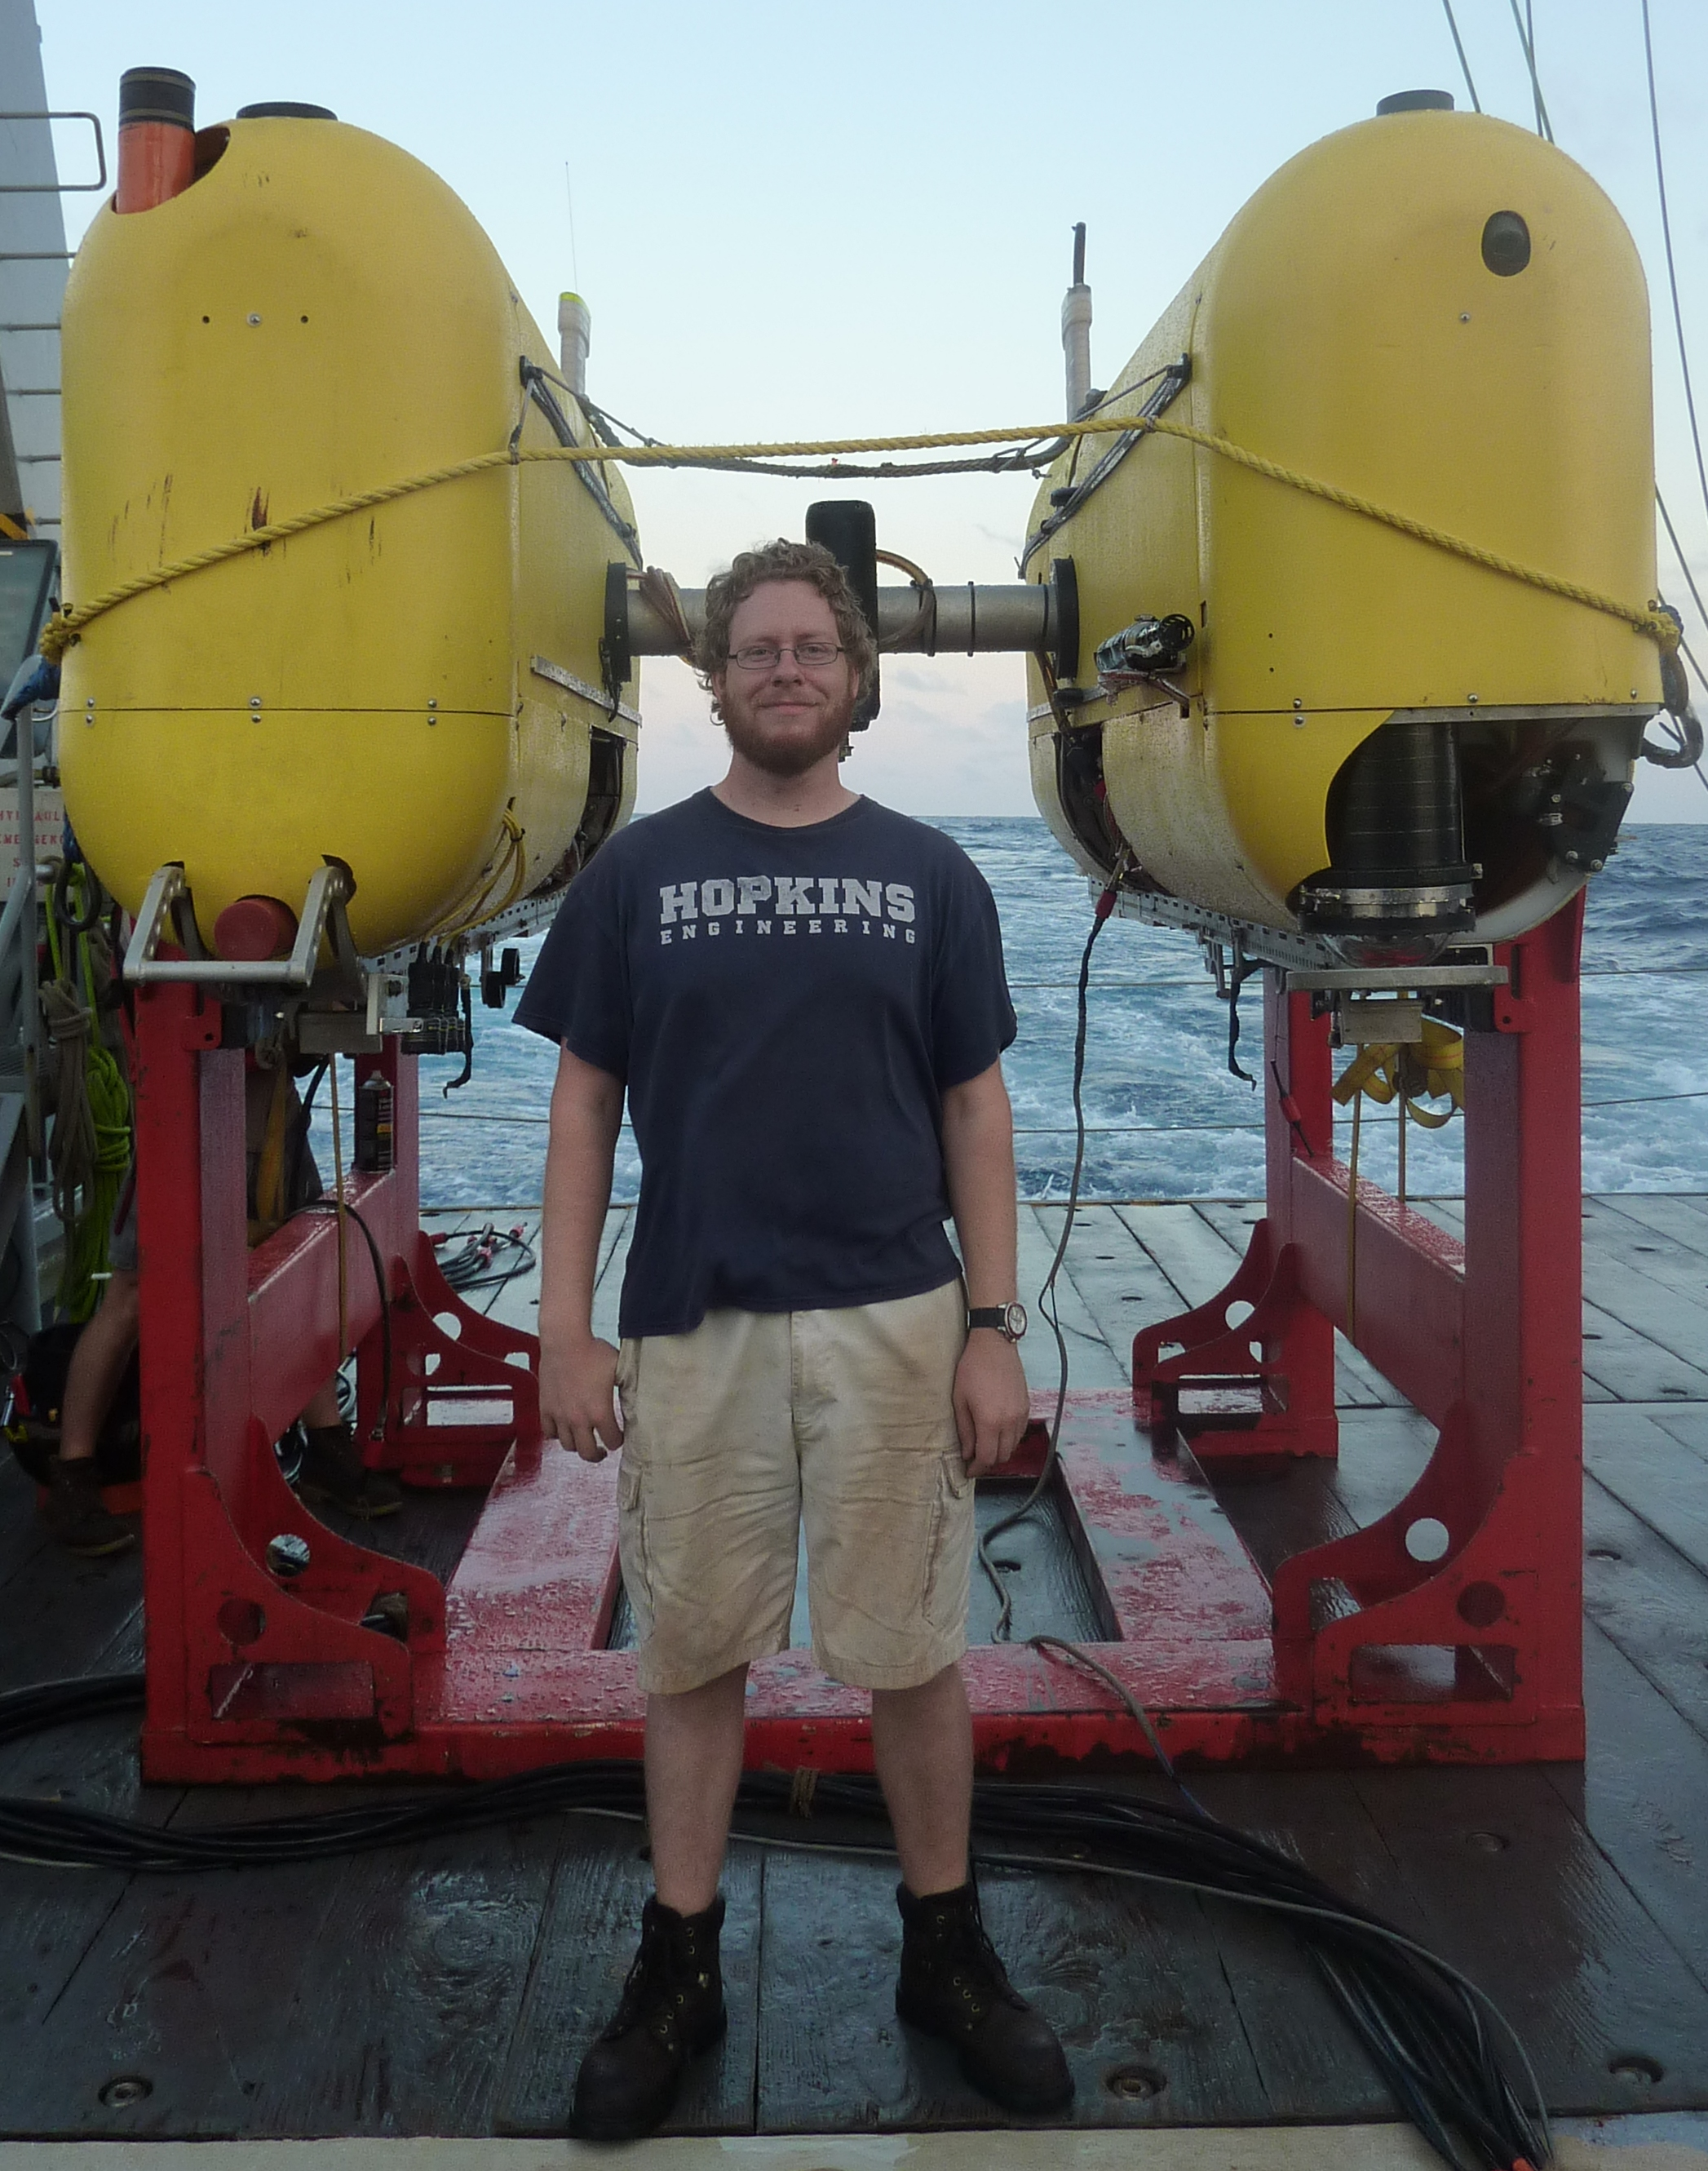
\includegraphics[width=40mm]{./pres/images/tophNereus}
%   \end{center}
%   \caption{McFarland and Nereus (WHOI) during field deployment in 2011.}
% \end{figure}
% \end{center}
% \end{columns}
% \end{frame}



% All of the following is optional and typically not needed. 
% \appendix
% \section<presentation>*{\appendixname}
% \subsection<presentation>*{For Further Reading}

% \begin{frame}[allowframebreaks]
%   \frametitle<presentation>{For Further Reading}
    
%   \begin{thebibliography}{10}
    
%   \beamertemplatebookbibitems
%   % Start with overview books.

%   \bibitem{Author1990}
%     A.~Author.
%     \newblock {\em Handbook of Everything}.
%     \newblock Some Press, 1990.
 
    
%   \beamertemplatearticlebibitems
%   % Followed by interesting articles. Keep the list short. 

%   \bibitem{Someone2000}
%     S.~Someone.
%     \newblock On this and that.
%     \newblock {\em Journal of This and That}, 2(1):50--100,
%     2000.
%   \end{thebibliography}
% \end{frame}
